
\section{Greedy Redundancy-based Cache Oblivious Data Layout Algorithm}

\subsection{Definitions}

For the purposes of this paper, we are given uniform data units in a linear sequence and each data unit has one or more access requirements assigned to it. An individual data unit consists of geometric primitive data or other information that must be retrieved during walkthrough rendering. The access requirements are determined by the application and represent data units that will be accessed together. An example of this could be vertices that are spatially near each other. \\
\\
For an access requirement $A$, the total span of $A$ is the total number of data units between the first and last data units that use $A$. If a data unit is not required by $A$ but lies between the first and last unit of $A$ then it is still counted in the span of $A$. Figure \ref{singleAR} shows a set of data units and explicitly labels the blue access requirement in this set. The total number of data units between the first and last blue unit is 14 thus that is the total length of the blue access requirement.\\
\\
\begin{figure}[ht]
\centering
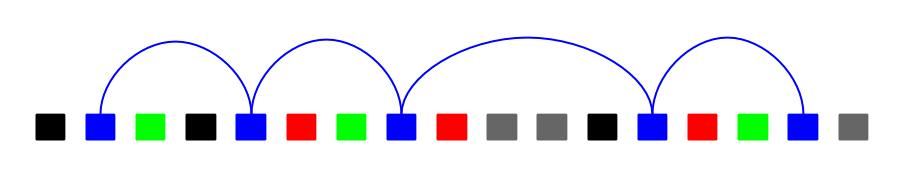
\includegraphics[width=3in]{SingleAR_start.jpg}
\caption{\YOON{Use PNG or some other formats that does not have much
compression artifacts.}Illustration of data units and a single access
requirement. The blocks are data units and the colors represent access
requirements. The curves connect data blocks with the same access requirement
and represent parts of the span of an access requirement.}
\label{singleAR}
\end{figure}

\YOON{This is a very important paragraph. I refined it, but it still comes
across weak to me.}
Instead of trying to find the seek time explicitly while
running, we use this
one dimensional layout to compute a probabilistic estimate for the seek time. A
cache-oblivious measure was introduced to measure the expected number of cache
misses~\cite{cacheobliviouslayout}. This measure is
based on the span of a simple access requirement consisting of two data access.
Note that every time we have cache misses, we would have to seek data from the
hard disk. We extend this idea by thinking of an individual cache miss as an
individual seek.
As a result, we define the Expected Seek Time (EST) as the total sum of
individual spans of access requirement.
%that could be required. 
Let $I$ be the set of access requirements and $A_i$
represent the span of access requirement $i$. 
%Because data units in an access
%requirement will be accessed together, 
We then have the following definition. 
\[
EST = \sum_{i \in I} A_i
\]

\YOON{We need to show some validation of this definition. Gopi mentioned that a prior work supported to use the span as a seek time. Can we mention that one here?}

\subsection{Algorithm Description}

In \cite{cacheobliviouslayout}, the only allowed operation on the data units is
the move operation and the optimal solution is computed using only that
operation. For our purposes, we are allowed to copy data units, move them, and
delete them if they are not used. We want to figure out how to minimize EST
while keeping the number of extra copies as low as possible. After constructing
a cache-oblivious layout to the mesh to get an initial optimization, we take a
data unit and copy it to a place that will shorten at least a span of the access
requirements that use it. If the new data unit reduces the span of all the
access requirements attached to it, then we delete the original data unit. We
repeat the individual copying and possible deletion procedure until our
redundancy limit has been reached. \\
\\
{\bf Blocks to consider:} Note that the span of an access requirement does not
change by moving an interior data unit to another interior location. Cost can
be reduced only by moving the blocks, i.e. data units, that are at the either ends of the access
requirement. This will greatly reduce the search space of data units to
consider for copying. For the sake of simplicity of the algorithm, we operate
on only one data block at a time. \\
\\
{\bf Location of copies:} Based on the above observation, given an access requirement, we can possibly move the beginning or the end data block of the access requirement to the interior and make it an interior block. This will reduce its span, thus reducing the EST for the layout. In order to maximize our benefit to our current access requirement, we want to copy the start data unit to somewhere between the one after the first one and the last one. In the same manner, we want to copy the end unit to somewhere between the first one and the one before the last one. \\
\\
Figure \ref{singleARafterCopy} shows the access requirement from the above figure (Fig.~\ref{singleAR}) with an arrow showing the locations where the start unit can be moved to as well as what the access requirement looks like after the copy. By moving it to one of the these locations we are guaranteed to reduce the span of the access requirement. The dashed line connects the original data unit with its copy. The solid blue lines in the bottom figure of Fig.~\ref{singleARafterCopy} represent the new span of the blue access requirement. Because the start unit has been copied and its copy is being used, it no longer is needed and is thus not counted in the new span for the blue access requirement. The span of the blue access requirement has been reduced from 14 units to 12 units.\\
\begin{figure}[ht]
\centering
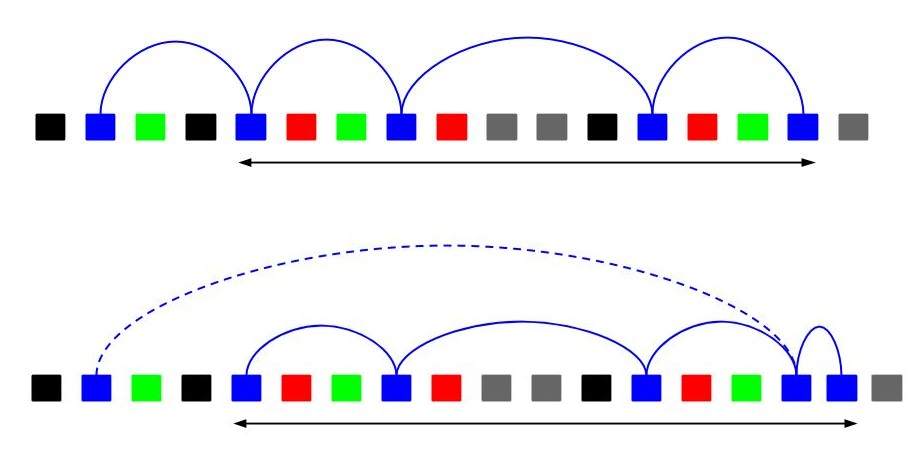
\includegraphics[width=3in]{SingleAR_afterCopy.jpg}
\caption{Interval where the start data unit can be copied to (top) and the data
units after the copy (bottom)
}
\label{singleARafterCopy}
\end{figure}
\\
For the access requirement under consideration, it does not matter where in the specified interval our data unit is moved. However, if the new location of the data block is in the span of other access requirements, it increases the span of those accesses by one unit. We thus want to find a location that is in the interior of the access requirement under consideration but is in the span of least number of access requirements. Such a location is identified using a simple linear search through the span of the access requirement. Figure \ref{singleARafterCopyOtherAR} shows the data units in figure \ref{singleAR} before the copying and highlights the gray access requirement that will be affected. As can be observed in figure \ref{singleARafterCopyOtherAR} the gray access requirement has had its span increased by 1. Even though we reduced the total span by 2 with the blue access requirement, we also increased the total span by 1 with the gray access requirement, yielding a net benefit of 1 data unit. If you search through all the spots in the interior of the blue access requirement, then the spot chosen had the least number of overlapping access requirements at 1.\\

\begin{figure}[ht]
\centering
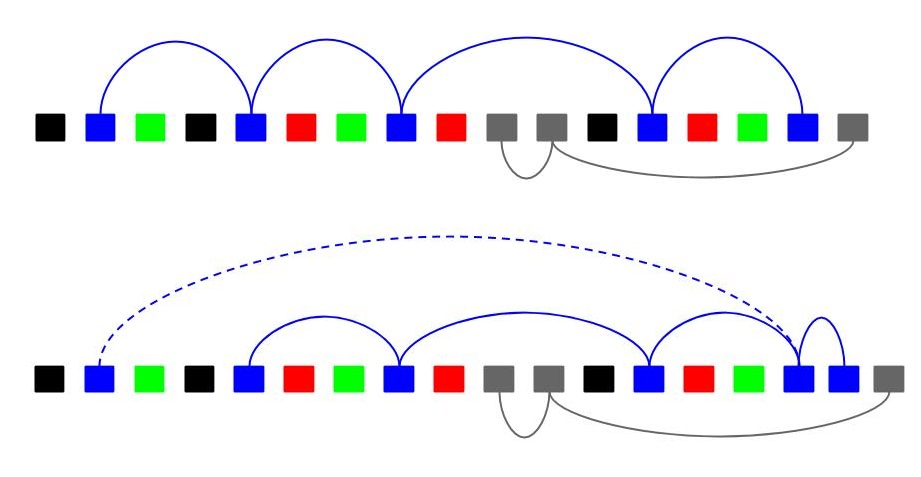
\includegraphics[width=3in]{SingleAR_afterCopy_otherARnoted.jpg}
\caption{The blue and gray access requirements before (top) and after (bottom) the copying}
\label{singleARafterCopyOtherAR}
\end{figure}

{\bf Moving versus Copying:} A data block can be accessed by multiple access
requirements. If that data block is an extremal block of access
requirements, and if it is moved to its interior, it affects span of those access
requirements that use the
same data block. That is the main reason that we are copying and not moving
these data blocks. By copying the data unit the other access requirements can
still access it in its old location without any change in their span.
Nevertheless, if by using the new copy the span of one or more of the other
access requirements reduces, then those access requirements should use the new
copy instead of the old copy. If all the access requirements use the new copy
and the old data block is not used by any access, then it can be deleted. In
this later case, we are really moving the data block. \\
\\
{\bf Data Block processing order:} 
We now need to figure out how to use this
information to decide in what order the copying should be done. For each data
unit, its total benefit is the amount that is reduces the total seek time
($EST$). For a given data unit to be copied to a specified location, let $k_i$
be the benefit to access requirement $i$ that is attached to the data unit. We
will say that $k_i=0$ if the access requirement will use the old copy and not have its span increased by the addition of a new copy, $k_i=-1$ if the access requirement will use the old copy but still have its span increased, and
$k_i>0$ if the access requirement will use the new copy. Let $I$ be the set of
access requirements that use the data unit. Let $J$ be the set of access
requirements not in $I$ whose span overlaps our data units. We can now describe
the benefit, the reduction in seek time, as follows:
\[
Benefit = -\Delta EST = \sum_{i \in I} k_i - |J|.
\]
Before doing any actual copying, we compute the above described benefit for
each start and end data unit for each access requirement. We store all the
benefits into a binary search tree, i.e. a heap, sorted in descending order by benefit
amount. That way we will easily be able to choose the data unit that provides
the most benefit in expected seek time. We will also make a special list $L$ of
cases where a data unit is copied and then can be deleted, because by doing
that, all the access
requirements will benefit. \\
\\
Because doing the moving for the list $L$ does not increase the storage, we will first go through that list and perform those moves. Once that list is empty we will take the data unit in the binary search tree that provides the most benefit and perform the copy. We will then recompute $L$ and the binary search tree. We will continue to do those steps until we have run out of available space for redundancy. As a summary, the psuedo-code of this algorithm is shown as algorithm \ref{pseudocode}.

\begin{algorithm}
Start with the data units which each with at least one access requirement (AR)\;
Initialize AR, heap H, and list L\;
\For{each data unit}{
	Find number of overlapping access requirements and store the number with the data unit\;
}
\For{each AR P's head and tail data units U}{
	make old copy list L' empty\;
	\eIf{U is head data unit}{
		Let S = data unit in P after U\;
	}{
		Let S = data unit in P before U\;
	}
	Set BENEFIT=distance(S,U)\;
	Let U' be the potential copy of U\;
	Search data units between S and U for min number of overlapping ARs and put U' there\;
	make old copy list L', the list that stores the ARs that will use the old data unit, empty\;
	\For{each AR T that also uses U}{
		\eIf{T will be shorter by using U'}{
			Add T's benefit to BENEFIT\;
		}{
			Add T to list L'\;
		}
	}
	Add BENEFIT to heap H\;
	\If{L' is empty}{
		add U to list L\;
	}
}
\While{BREAK has not been called}{
		\While{L is not empty}{
			Take out random element and move the data unit\;
			Update heap H and list L\;
		}
		\eIf{there is more space for redundancy}{
		pop best element U from H\;
		copy U to its destination\;
		update nodes in H and entries in L for affected access requirements\;
		update H and L\;
		}{ call BREAK}
}
\caption{Pseudo-code for our algorithm}
\label{pseudocode}
\end{algorithm}

